\documentclass{article}

% Language setting
% Replace `english' with e.g. `spanish' to change the document language
\usepackage[english]{babel}

% Set page size and margins
% Replace `letterpaper' with `a4paper' for UK/EU standard size
\usepackage[letterpaper,top=2cm,bottom=2cm,left=3cm,right=3cm,marginparwidth=1.75cm]{geometry}
\usepackage{CJKutf8}
% Useful packages
\usepackage{amsmath}
\usepackage{graphicx}
\usepackage{setspace}
\usepackage{float}
\usepackage{subfigure}
\usepackage[section]{placeins}
\usepackage[colorlinks=true, allcolors=blue]{hyperref}
\usepackage[export]{adjustbox}

\author{B10209040 陳彥倫}

\begin{document}
\thispagestyle{empty}
\hfill {\scshape \large Cloud Physics, Fall 2023 } \hfill {\scshape P1}
\smallskip
\hrule
\begin{CJK*}{UTF8}{bsmi}
\bigskip
\bigskip
\bigskip

\centerline{\huge \textbf {HW2}}
\bigskip
\centerline{\textbf {B10209040 陳彥倫}}

\section*{1.}
\begin{spacing}{2}
    \begin{large}
        \textbf{For Bowen's model:} \\
        \centerline{$\frac{dR}{dt} = \frac{\overline{E}\cdot L}{4\rho_w} \cdot u(R)$} \\
        \centerline{$\frac{dR}{dt} = \frac{dR}{dt} \frac{dt}{dz} = \frac{\overline{E}\cdot L}{4\rho_w} \cdot u(R) \cdot \frac{1}{w - u(R)}$} \\
        with $\overline{E} = 1, L = 2.5g \cdot m^{-3}, u(R) = aR^b, $ where $a = 8500, b = 1 $
    \end{large}
\end{spacing}


\subsection*{(1)}
\begin{spacing}{1.5}
    \begin{large}
        \centerline{Case A: 2.003 mm , Case B: 0.806 mm }
        \centerline{Case C: 4.875 mm , Case D: 2.004 mm }
        \; \\
            由上述公式推導及觀察可得雨滴的半徑及終端速度在一開始會隨著高度上升而增加。而終端速度的絕對值一旦增加至大
            於雨滴初始的上升速度時,雨滴的高度即開始下降。將時步設置為1sec, 利用迭代法計算出雨滴在半徑、時間、高度變
            化的過程,求z序列第二次等於0的時候可得上述結果(因無剛好等於0之資料點,取最接近之值)。
    \end{large}
\end{spacing}

%\newpage

\subsection*{(2)}
\begin{figure}[!htbp]
    \centering
    \subfigure[Height - time]{
    \begin{minipage}[t]{0.5\linewidth}
    \centering
    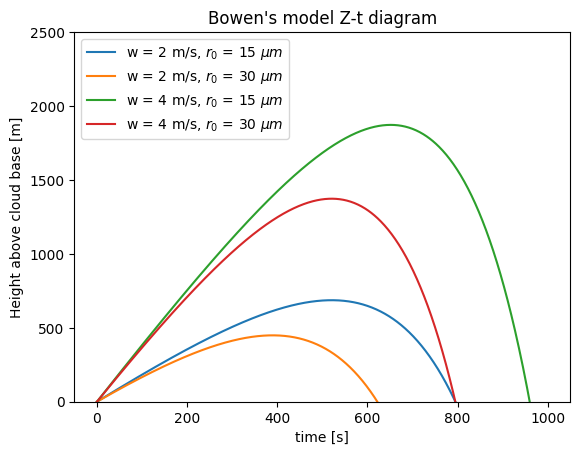
\includegraphics[scale=0.4]{zt.png}
    %\caption{fig1}
    \end{minipage}%
    }%
    \subfigure[Height - radius]{
    \begin{minipage}[t]{0.5\linewidth}
    \centering
    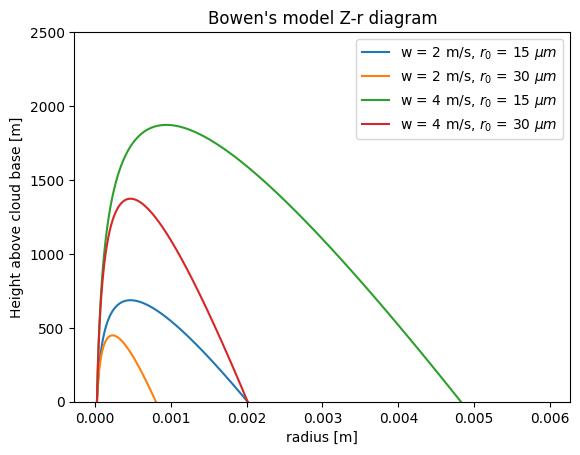
\includegraphics[scale=0.4]{zr.png}
    %\caption{fig2}
    \end{minipage}%
    }%
\end{figure}

\newpage
\thispagestyle{empty}
\hfill {\scshape \large Cloud Physics, Fall 2023 } \hfill {\scshape P2}
\smallskip
\hrule
\bigskip
\subsection*{(3)}
    \begin{spacing}{1.5}
        \begin{large}
            觀察(a)之軌跡圖可以驗證前述數學式導出的雨滴隨時間變化會逐漸上升最後落回地面的現象。分別比較不同上升速度及不同
            初始半徑大小,在上升的最高高度方面,具有較大上升速度及較小初始半徑的水滴能夠在雲中上升至較高處才開始下墜。落回
            地面的時間則以case B 和 case C較接近,可知上升速度越大,體積越小之雨滴能在雲底上方停留較長時間。(b)圖表雨滴
            半徑成長隨高度變化的趨勢與軌跡相似,不同的是圖形初始的斜率較大,表示剛開始半徑成長較快速。
        \end{large}
    \end{spacing}
\subsubsection*{Comparison:}
    \begin{spacing}{1.5}
        \begin{large}
            與投影片中文獻的圖片相比,形狀及高度相近,但時間規模差異較大,可能為計算方式或常數設定不同所造成。
        \end{large}
    \end{spacing}
    




\end{CJK*}
\end{document}